%!TEX TS-program = xelatex
\documentclass[12pt, a4paper]{article}  

\usepackage{etex} % расширение классического tex в частности позволяет подгружать гораздо больше пакетов, чем мы и займёмся далее

%%%%%%%%%% Математика %%%%%%%%%%
\usepackage{amsmath,amsfonts,amssymb,amsthm,mathtools} 
%\mathtoolsset{showonlyrefs=true}  % Показывать номера только у тех формул, на которые есть \eqref{} в тексте.
%\usepackage{leqno} % Нумерация формул слева


%%%%%%%%%%%%%%%%%%%%%%%% Шрифты %%%%%%%%%%%%%%%%%%%%%%%%%%%%%%%%%
\usepackage{fontspec}         % пакет для подгрузки шрифтов
\setmainfont{Arial}   % задаёт основной шрифт документа

\defaultfontfeatures{Mapping=tex-text}

% why do we need \newfontfamily:
% http://tex.stackexchange.com/questions/91507/
\newfontfamily{\cyrillicfonttt}{Arial}
\newfontfamily{\cyrillicfont}{Arial}
\newfontfamily{\cyrillicfontsf}{Arial}

\usepackage{unicode-math}     % пакет для установки математического шрифта
\setmathfont{Asana Math}      % шрифт для математики
% \setmathfont[math-style=ISO]{Asana Math}
% Можно делать смену начертания с помощью разных стилей

% Конкретный символ из конкретного шрифта
% \setmathfont[range=\int]{Neo Euler}

\usepackage{polyglossia}      % Пакет, который позволяет подгружать русские буквы
\setdefaultlanguage{russian}  % Основной язык документа
\setotherlanguage{english}    % Второстепенный язык документа


%%%%%%%%%% Работа с картинками %%%%%%%%%
\usepackage{graphicx}                  % Для вставки рисунков
\usepackage{graphics}
\graphicspath{{images/}{pictures/}}    % можно указать папки с картинками
\usepackage{wrapfig}                   % Обтекание рисунков и таблиц текстом
\usepackage{subfigure}                 % для создания нескольких рисунков внутри одного


%%%%%%%%%% Работа с таблицами %%%%%%%%%%
\usepackage{tabularx}            % новые типы колонок
\usepackage{tabulary}            % и ещё новые типы колонок
\usepackage{array}               % Дополнительная работа с таблицами
\usepackage{longtable}           % Длинные таблицы
\usepackage{multirow}            % Слияние строк в таблице
\usepackage{float}               % возможность позиционировать объекты в нужном месте
\usepackage{booktabs}            % таблицы как в книгах!
\renewcommand{\arraystretch}{1.3} % больше расстояние между строками

% Заповеди из документации к booktabs:
% 1. Будь проще! Глазам должно быть комфортно
% 2. Не используйте вертикальные линни
% 3. Не используйте двойные линии. Как правило, достаточно трёх горизонтальных линий
% 4. Единицы измерения - в шапку таблицы
% 5. Не сокращайте .1 вместо 0.1
% 6. Повторяющееся значение повторяйте, а не говорите "то же"
% 7. Есть сомнения? Выравнивай по левому краю!

%%%%%%%%%% Графика и рисование %%%%%%%%%%
\usepackage{tikz, pgfplots}  % язык для рисования графики из latex'a
\usepackage{amscd}                  %Пакеты для рисования
\usepackage[matrix,arrow,curve]{xy} %комунитативных диаграмм

% Всякие странные команды из Geogebra и с сайта для TikZ
\usepackage{pgf}
\usepackage{mathrsfs}
\usetikzlibrary{arrows}
\pagestyle{empty}

\definecolor{ffzzzz}{rgb}{1.,0.6,0.6}
\definecolor{xdxdff}{rgb}{0.49019607843137253,0.49019607843137253,1.}
\definecolor{qqqqff}{rgb}{0.,0.,1.}
\definecolor{cqcqcq}{rgb}{0.7529411764705882,0.7529411764705882,0.7529411764705882}

\usetikzlibrary{calc}
\usepackage{relsize}
\newcommand\LM{\ensuremath{\mathit{LM}}}
\newcommand\IS{\ensuremath{\mathit{IS}}}




\title{Графика в LaTeX, TikZ}
\date{\today}



\begin{document} % конец преамбулы, начало документа


\section{Внутренние средства для графики в \LaTeX{} или как не надо делать!}


\begin{center}
\begin{picture}(200,100)
\put(50,50){\oval(50,100)}
\put(150,50){\oval(50,100)}
\put(50,80){\circle*{2}}
\put(43,80){\footnotesize{1}}
\put(50,60){\circle*{2}}
\put(43,60){\footnotesize{2}}
\put(50,40){\circle*{2}}
\put(43,40){\footnotesize{3}}
\put(50,20){\circle*{2}}
\put(43,20){\footnotesize{4}}
\put(150,80){\circle*{2}}
\put(153,80){\footnotesize{5}}
\put(150,60){\circle*{2}}
\put(153,60){\footnotesize{11}}
\put(150,40){\circle*{2}}
\put(153,40){\footnotesize{12}}
\put(150,20){\circle*{2}}
\put(153,20){\footnotesize{17}}
\put(53,80){\vector(1,0){94}}
\put(147,80){\vector(-1,0){94}}
\put(53,60){\vector(1,0){94}}
\put(147,60){\vector(-1,0){94}}
\put(53,40){\vector(1,0){94}}
\put(147,40){\vector(-1,0){94}}
\put(53,20){\vector(1,0){94}}
\put(147,20){\vector(-1,0){94}}
\end{picture}
\end{center}

\begin{figure}[h!]
\begin{center}
\[ \xymatrix{
(1,1) \ar[r] &  (1,2) \ar[ld]  &  (1,3) \ar[r]  & (1,4) \ar[ld]  & (1,5)  \ar[r] & \dots  \\
(2,1) \ar[d] & (2,2) \ar[ru]  & (2,3) \ar[ld]  & (2,4) \ar[ur] & (2,5) &  \dots\\
(3,1) \ar[ru] & (3,2) \ar[ld] & (3,3) \ar[ur] & (3,4) & (3,5)  & \dots \\
(4,1) \ar[d] & (4,2) \ar[ur] & (4,3) & (4,4) & (4,5)  & \dots \\
(5,1) \ar[ur] & (5,2) & (5,3) & (5,4) & (5,5)  & \dots \\
\dots & \dots & \dots & \dots & \dots  }
\]
\caption{Нумерация элементов в множестве пар натуральных чисел $\mathbb{N}^2$}\label{n^2}
\end{center}
\end{figure}


\newpage 

\section{Великий и могучий Tikz}
\subsection{ Основные команды} 


% Никогда не забывать в конце каждой строки ставить ;
% Tikz очень капризен по отношению к этому!

\begin{center}
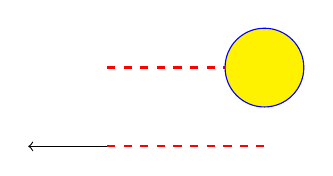
\begin{tikzpicture}
\draw[red, dashed, thick] (0,1) -- (2,1) (0,2) -- (2,2);
\draw[->] (0,1) -- (-1,1);
\draw[blue,fill=yellow](2,2) circle [radius = 0.5];
\end{tikzpicture}
\end{center}

\vspace{1cm}

\begin{tikzpicture}
\foreach \x in {0,...,9}
  \draw [->] (\x,0)--(\x,-1);
\end{tikzpicture}

\vspace{1cm}

%\draw [domain=<xmin>:<xmax>] plot (\x, {function})

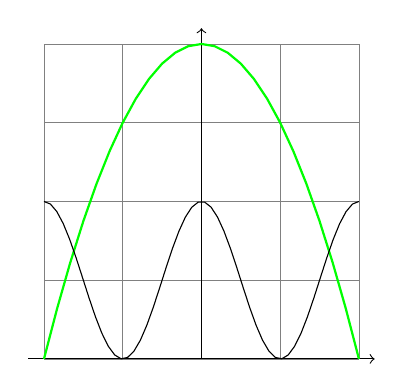
\begin{tikzpicture}
\draw [help lines] (-2,0) grid (2,4); 
\draw [->] (-2.2,0) -- (2.2,0); 
\draw [->] (0,0) -- (0,4.2); 
\draw [green, thick, domain=-2:2] plot (\x, {4-\x*\x}); 
\draw [domain=-2:2, samples=50] plot (\x, {1+cos(pi*\x r});
\end{tikzpicture}


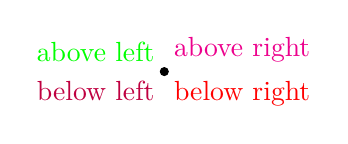
\begin{tikzpicture}[scale=2]
\draw[fill] (0.5,0.75) circle [radius=0.025];
\node [below right, red] at (0.5,0.75) {below right};
\node [above left, green] at (0.5,0.75) {above left};
\node [below left, purple] at (0.5,0.75) {below left};
\node [above right, magenta] at (0.5,0.75) {above right};
\end{tikzpicture}
% измнение scale не изменяет размер текста


\subsection{Tikztempaltes и их редактирование}

% Пример взят отсюда!
% http://www.texample.net/tikz/examples/is-lm-diagram/

\begin{figure}[h]
\begin{center}
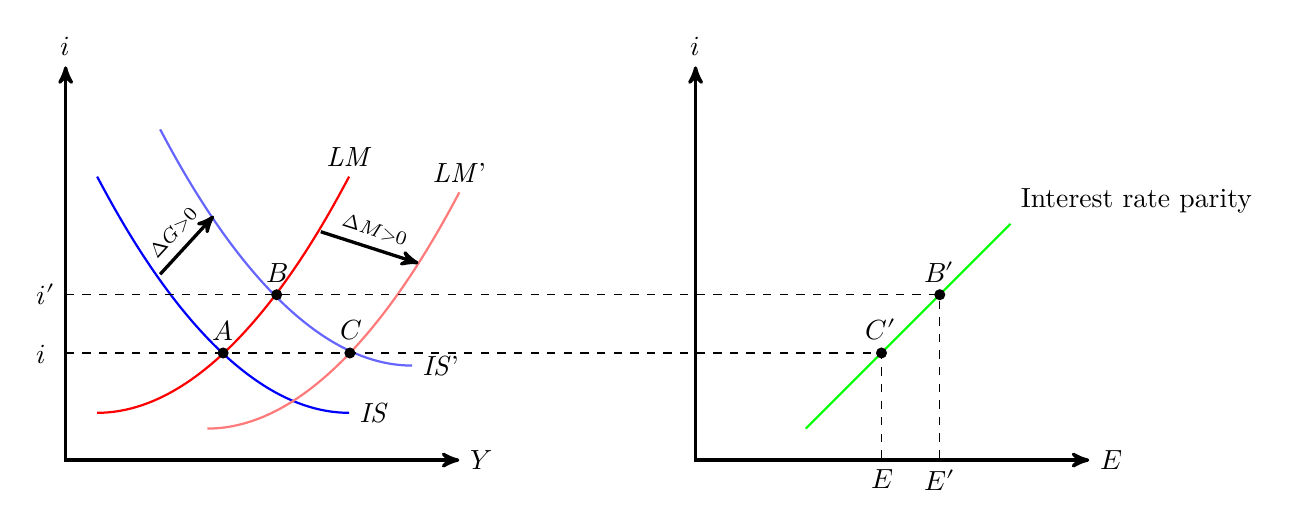
\begin{tikzpicture}[
        scale=2,
        IS/.style={blue, thick},
        LM/.style={red, thick},
        axis/.style={very thick, ->, >=stealth', line join=miter},
        important line/.style={thick}, dashed line/.style={dashed, thin},
        every node/.style={color=black},
        dot/.style={circle,fill=black,minimum size=4pt,inner sep=0pt,
            outer sep=-1pt},
    ]
    % axis
    \draw[axis,<->] (2.5,0) node(xline)[right] {$Y$} -|
                    (0,2.5) node(yline)[above] {$i$};
    % IS-LM diagram
    \draw[LM] (0.2,0.3) coordinate (LM_1) parabola (1.8,1.8)
        coordinate (LM_2) node[above] {\LM};
    \draw[IS] (0.2,1.8) coordinate (IS_1) parabola[bend at end]
         (1.8,.3) coordinate (IS_2) node[right] {\IS};
    %Intersection is calculated "manually" since Tikz does not offer
    %intersection calculation for parabolas
    \node[dot,label=above:$A$] at (1,.68) (int1) {};
    %shifted IS-LM diagram
    \draw[xshift=.7cm, LM, red!52] (0.2,0.2) parabola (1.8,1.7)
        node[above] {\LM'};
    \draw[xshift=.4cm, yshift=.3cm, IS, blue!60] (0.2,1.8)
        parabola[bend at end] (1.8,.3)
        node[right] {\IS'};
    %Intersection of shifted IS-LM
    \path[xshift=.36cm, yshift=.35cm] (.98,.7)
        node[dot,label=above:{$B$}] (int2) {};
    \path[xshift=.805cm] (1,.68) node[dot,label=above:$C$] (int3) {};
    %arrows between intersections
    \draw[->, very thick, black, >=stealth']
        ($(int1)+1/2*(-.80,1)$) -- ($(int2)+1/2*(-.8,1)$)
        node[sloped, above, midway] {$\mathsmaller{\Delta G > 0}$};
    \draw[->, very thick, black, >=stealth']
        ($(int2)+2*(.14,.2)$) -- ($(int2)!.2cm!270:(int2)+(.9,0)$)
        node[sloped,above, midway] {$\mathsmaller{\Delta M>0}$};
        
    \begin{scope}[xshift=4cm]
        %E-diagram
        \draw[axis,<->] (0,2.5) node(eyline)[above] {$i$} |-
                        (2.5,0) node(exline)[right] {$E$};

        \draw[important line, green, xshift=.5cm]
            (.2,.2) coordinate (es) -- (1.5,1.5) coordinate (ee)
            node [above right] {Interest rate parity};
    \end{scope}
    %Lines connecting IS LM coordinates and E coordinates
    \draw[dashed] 
        let
            % Store the intersection point in \p1 for later retrieval. 
            % A convenient feature of the let operation is that we can
            % access the x and y component of the coordinate directly 
            % using the \x1 and \y1 syntax. 
            \p1=(intersection of int2--[xshift=1]int2 and es--ee)
        in
            (0,\y1) node[left]{$i'$} -|  (\x1,0)
            node[pos=0.5,dot,label=above:$B'$] {} node[below] {$E'$};

    \draw[dashed line] let
        \p1=(intersection of int3--[xshift=1]int3 and es--ee)
            in
        (0,\y1) node[left]{$i\phantom{'}$} -| (\x1,0)
        node[dot,label=above:$C'$,pos=0.5] {} node[below] {$E$};

\end{tikzpicture}
\end{center}
\caption{Модель IS-LM }
\end{figure}

\subsection{Geogebra}

\begin{center}
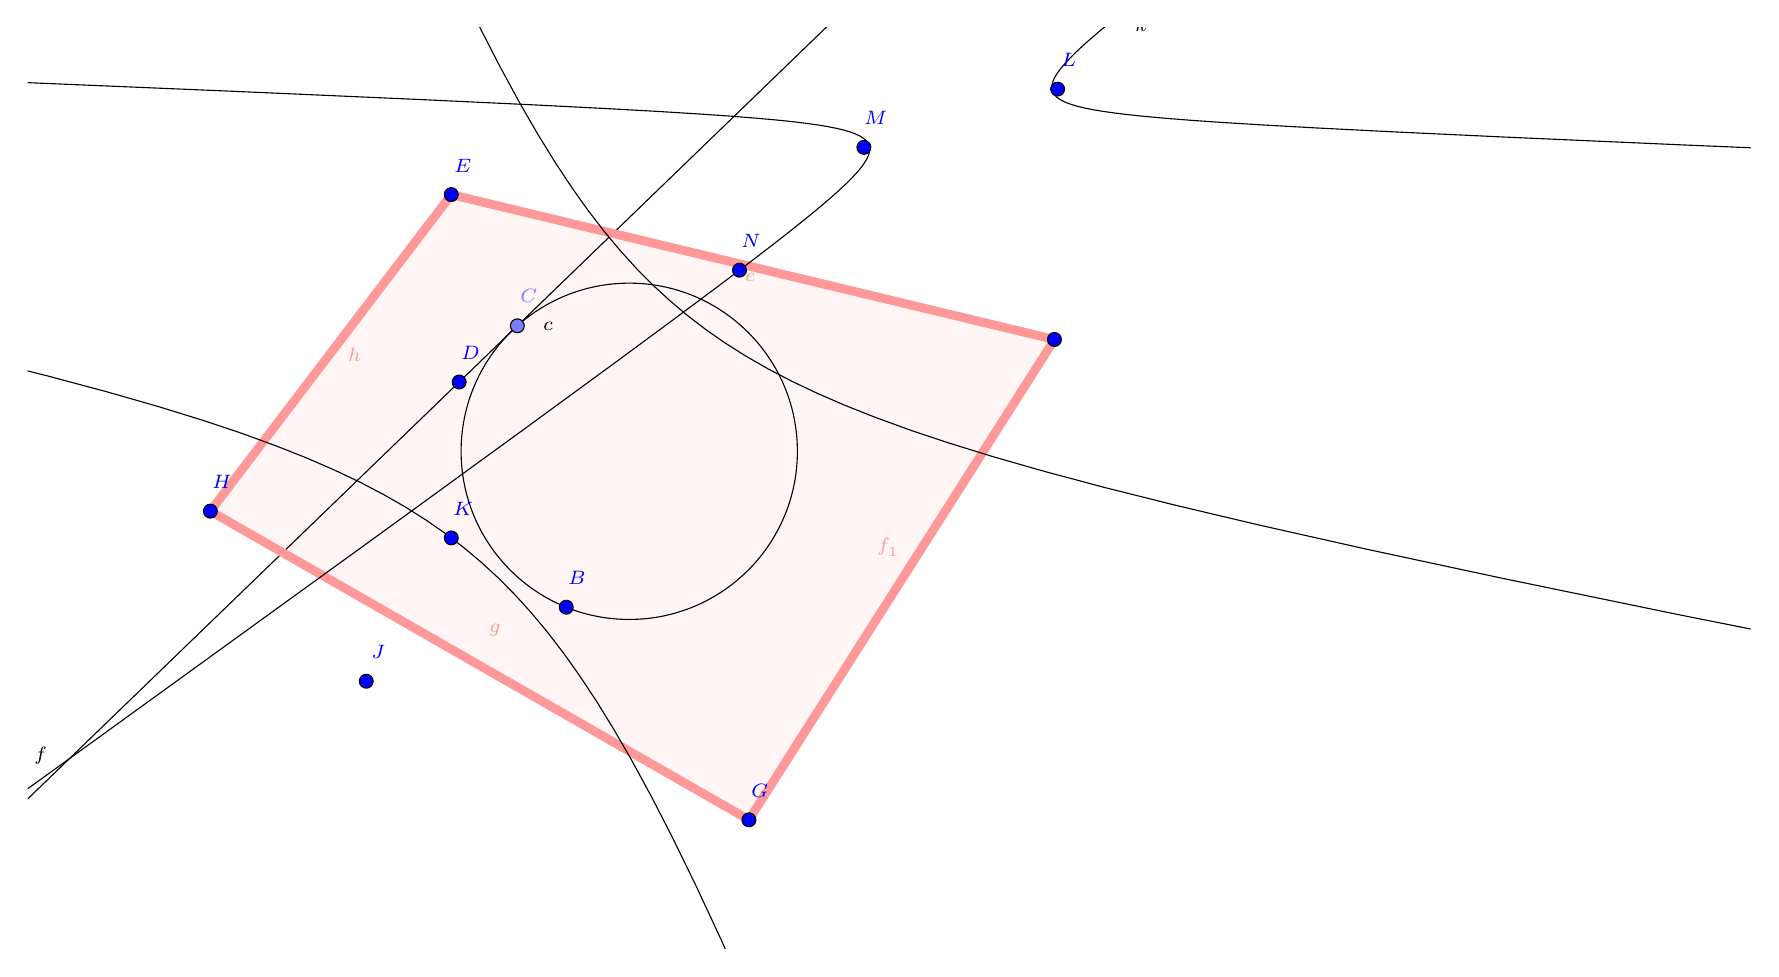
\begin{tikzpicture}[line cap=round,line join=round,>=triangle 45,x=1.0cm,y=1.0cm]

\clip(-4.3,-5.4) rectangle (17.58,6.3);
\fill[line width=3.2pt,color=ffzzzz,fill=ffzzzz,fill opacity=0.10000000149011612] (1.08,4.18) -- (8.74,2.34) -- (4.86,-3.76) -- (-1.98,0.16) -- cycle;
\draw(3.34,0.92) circle (2.135509306933594cm);
\draw [domain=-4.3:17.58] plot(\x,{(-0.48745752371228157-0.7139786516045719*\x)/-0.7388624070031535});
\draw [line width=3.2pt,color=ffzzzz] (1.08,4.18)-- (8.74,2.34);
\draw [line width=3.2pt,color=ffzzzz] (8.74,2.34)-- (4.86,-3.76);
\draw [line width=3.2pt,color=ffzzzz] (4.86,-3.76)-- (-1.98,0.16);
\draw [line width=3.2pt,color=ffzzzz] (-1.98,0.16)-- (1.08,4.18);
\draw [samples=50,domain=-0.99:0.99,rotate around={49.99942546060279:(2.66,1.17)},xshift=2.66cm,yshift=1.17cm] plot ({2.0405506305141534*(1+(\x)^2)/(1-(\x)^2)},{3.600090710566651*2*(\x)/(1-(\x)^2)});
\draw [samples=50,domain=-0.99:0.99,rotate around={49.99942546060279:(2.66,1.17)},xshift=2.66cm,yshift=1.17cm] plot ({2.0405506305141534*(-1-(\x)^2)/(1-(\x)^2)},{3.600090710566651*(-2)*(\x)/(1-(\x)^2)});
\draw [samples=50,domain=-0.99:0.99,rotate around={16.7419703852931:(7.55,5.15)},xshift=7.55cm,yshift=5.15cm] plot ({1.2142337390632962*(1+(\x)^2)/(1-(\x)^2)},{0.4188513183941076*2*(\x)/(1-(\x)^2)});
\draw [samples=50,domain=-0.99:0.99,rotate around={16.7419703852931:(7.55,5.15)},xshift=7.55cm,yshift=5.15cm] plot ({1.2142337390632962*(-1-(\x)^2)/(1-(\x)^2)},{0.4188513183941076*(-2)*(\x)/(1-(\x)^2)});
\begin{scriptsize}
\draw [fill=qqqqff] (2.54,-1.06) circle (2.5pt);
\draw[color=qqqqff] (2.68,-0.69) node {$B$};
\draw[color=black] (2.32,2.51) node {$c$};
\draw [fill=xdxdff] (1.9188624070031535,2.513978651604572) circle (2.5pt);
\draw[color=xdxdff] (2.06,2.89) node {$C$};
\draw [fill=qqqqff] (1.18,1.8) circle (2.5pt);
\draw[color=qqqqff] (1.32,2.17) node {$D$};
\draw[color=black] (-4.14,-2.95) node {$f$};
\draw [fill=qqqqff] (1.08,4.18) circle (2.5pt);
\draw[color=qqqqff] (1.22,4.55) node {$E$};
\draw [fill=qqqqff] (8.74,2.34) circle (2.5pt);
\draw [fill=qqqqff] (4.86,-3.76) circle (2.5pt);
\draw[color=qqqqff] (5.,-3.39) node {$G$};
\draw [fill=qqqqff] (-1.98,0.16) circle (2.5pt);
\draw[color=qqqqff] (-1.84,0.53) node {$H$};
\draw[color=ffzzzz] (4.88,3.13) node {$e$};
\draw[color=ffzzzz] (6.63,-0.3) node {$f_1$};
\draw[color=ffzzzz] (1.64,-1.35) node {$g$};
\draw[color=ffzzzz] (-0.14,2.15) node {$h$};
\draw [fill=qqqqff] (0.,-2.) circle (2.5pt);
\draw[color=qqqqff] (0.14,-1.63) node {$J$};
\draw [fill=qqqqff] (1.08,-0.18) circle (2.5pt);
\draw[color=qqqqff] (1.22,0.19) node {$K$};
\draw[color=black] (0.96,8.13) node {$d$};
\draw [fill=qqqqff] (8.78,5.52) circle (2.5pt);
\draw[color=qqqqff] (8.92,5.89) node {$L$};
\draw [fill=qqqqff] (6.32,4.78) circle (2.5pt);
\draw[color=qqqqff] (6.46,5.15) node {$M$};
\draw [fill=qqqqff] (4.74,3.22) circle (2.5pt);
\draw[color=qqqqff] (4.88,3.59) node {$N$};
\draw[color=black] (9.84,6.33) node {$k$};
\end{scriptsize}
\end{tikzpicture}
\end{center}

\end{document} % конец документа